\documentclass[crop,tikz]{standalone}% 'crop' is the default for v1.0, before it was 'preview'
\usepackage{tikz,calc,pgfplots}
\usetikzlibrary{calc}
\begin{document}
	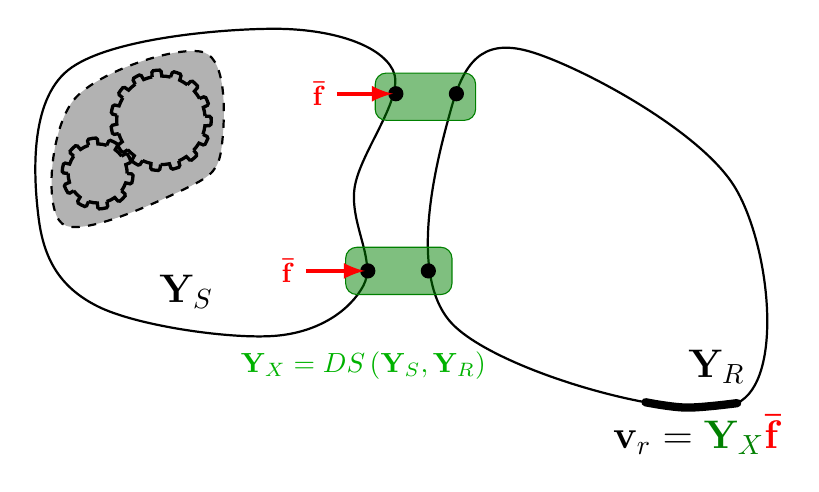
\begin{tikzpicture}[scale=0.75]
		\draw [thick]  plot[smooth cycle, tension=.6] coordinates {(0,2) (0.5,4.5) (4,5.2) (6,4.5)  (5.35,2.5) (5.5,0.85) (4,0) (1,0.5) };
		\node[outer sep=0pt,thick] at (2.5,0.75) [] {\Large${\mathbf{Y}_S}$};
		
		
		
		\newcommand{\gear}[5]{%
			\foreach \i in {1,...,#1}
			{   [rotate=(\i-1)*360/#1] (0:#2) arc (0:#4:#2) {[rounded corners=0.5pt] -- (#4+#5:#3)  arc (#4+#5:360/#1-#5:#3)} --  (360/#1:#2)
			}
		}  
		
		% given
		\pgfmathsetmacro{\rOne}{0.5}% inner radius
		\pgfmathsetmacro{\nOne}{10}% num teeth
		\pgfmathsetmacro{\nTwo}{15}
		\pgfmathsetmacro{\toothHeight}{0.1}
		\pgfmathsetmacro{\toothFall}{1}% degrees where radius drops from inner to outer
		\pgfmathsetmacro{\aOneTwo}{40}% angle from first to second
		
		% computed
		\pgfmathsetmacro{\rTwo}{\rOne*\nTwo/\nOne}% via equating tooth lengths
		\pgfmathsetmacro{\ROne}{\rOne+\toothHeight}% outer radius
		\pgfmathsetmacro{\RTwo}{\rTwo+\toothHeight}
		\pgfmathsetmacro{\dOne}{(360/\nOne-\toothFall)/2}% degrees for a tooth; here inner deg = outer deg
		\pgfmathsetmacro{\dTwo}{(360/\nTwo-\toothFall)/2}
		\pgfmathsetmacro{\distOneTwo}{\rOne+\rTwo+\toothHeight+0.05}
		
		
%		\draw [-stealth,line width=1pt,red] (2.8,2.9) -- ($(2.8,2.9)+(0.7, -0.7)$); 
%		\draw [-stealth,line width=1pt,red] (2.8,4.5) -- ($(2.8,4.5)+(1, 0.1)$) ; 
%		\draw [-stealth,line width=1pt,red] (2.8,3.5) -- ($(2.8,3.5)+(1, 0.1)$) ; 
%		\draw [-stealth,line width=1pt,red] (2.5,2.5) -- ($(2.5,2.5)+(0.25, -0.7)$) ; 
%		\draw [-stealth,line width=1pt,red] (1,3) -- ($(1,3) +(0.2, -2)$) ; 
%		\draw [-stealth,line width=1pt,red] (1.7,3) -- ($(1.7,3) +(0.3, -2)$) ; 
		
		\draw [thick, dashed,fill=white!70!black,]  plot[smooth cycle,  tension=.6] coordinates {(0.4,1.9) (.6,4) (2.8,4.8)  (3.1,3.2) (2.5,2.5) };
		
		
		\begin{scope}[shift={(1.,2.75)}]
			\draw[very thick,,] \gear{\nOne}{\rOne}{\ROne}{\dOne}{\toothFall};
			\draw[very thick, ,shift={(\aOneTwo:\distOneTwo)}, rotate=5.5] \gear{\nTwo}{\rTwo}{\RTwo}{\dTwo}{\toothFall};
		\end{scope}
		
		
		\begin{scope}[xshift=7.25cm,yshift=4.8cm, rotate=-15.5]
			\draw [thick]  plot[smooth cycle, tension=.6] coordinates {(0,-1) (1,-4.5) (6,-4.5) (5,-1) (1,0.3) };
			\node[outer sep=0pt,thick] at (5.5,-4) [] {\Large${\mathbf{Y}_R}$};
			
			\draw [line width=3pt,black,cap=round]  plot[smooth, tension=.6] coordinates {  (6,-4.5) (5.2,-4.8) (4.5,-4.9) };  
			\node[outer sep=0pt,thick] at (5.5,-5.2) [] {\Large$\mathbf{v}_r = {\color{green!50!black}\mathbf{Y}_X } {\color{red} \mathbf{\bar{f}}}$};
		\end{scope}
		
		 \draw[rounded corners, rotate=0, fill=green!50!black, fill opacity=0.5, green!50!black, shift={(0.9,-0.45)}] (4.8,4.1)rectangle (6.5,4.9) {};
		
		\draw[rounded corners, rotate=0, fill=green!50!black, fill opacity=0.5, green!50!black, shift={(0.9,-0.45)}] (4.3,1.15)rectangle (6.1,1.95) {};
		
		\node[outer sep=0pt,thick] at (5.5,-0.5) [] {$\color{green!70!black}\mathbf{Y}_X = {DS}\left(\mathbf{Y}_{S},\mathbf{Y}_{R}\right) $};
		
		\begin{scope}[xshift=1.025cm]
			\draw[very thick, black, fill=black] (6.05,4.1) circle[radius=.1];
			
			\draw[very thick, black, fill=black] (5.575,1.1) circle[radius=.1];
		\end{scope}
		
		\draw[very thick, black, fill=black] (6.05,4.1) circle[radius=.1];
		
		\draw[very thick, black, fill=black] (5.575,1.1) circle[radius=.1];
%		\node[outer sep=0pt,thick] at (6.2,5) [] {\Large$c$};
		
		\draw[red,-latex,ultra thick] (5.05,4.1)--(6.,4.1) node [pos=0,left] {$\mathbf{\bar{f}}$};
		
		\draw[red,-latex,ultra thick] (4.525,1.1)--(5.525,1.1)  node [pos=0,left] {$\mathbf{\bar{f}}$};
		
		
	\end{tikzpicture}
\end{document}